\documentclass[aspectratio=169,12pt,t]{beamer}

% --- Theme: Metropolis (modern, clean) ---
\usetheme[progressbar=frametitle,numbering=fraction,block=fill]{metropolis}

% --- Fira Sans font (install texlive-fonts-extra if missing) ---
\IfFileExists{FiraSans.sty}{\usepackage[sfdefault]{FiraSans}}{}

% --- Light background with warm accent ---
\definecolor{mDarkTeal}{RGB}{35,55,59}
\definecolor{mLightBrown}{RGB}{235,228,216}
\definecolor{mAccent}{RGB}{140,70,20}

\setbeamercolor{normal text}{fg=mDarkTeal,bg=white}
\setbeamercolor{alerted text}{fg=mAccent}
\setbeamercolor{frametitle}{bg=mDarkTeal,fg=white}
\setbeamercolor{progress bar}{fg=mAccent,bg=mLightBrown}
\setbeamercolor{title separator}{fg=mAccent}
\setbeamercolor{progress bar in head/foot}{fg=mAccent,bg=mLightBrown}
\setbeamercolor{progress bar in section page}{fg=mAccent,bg=mLightBrown}

% --- Packages ---
\usepackage[utf8]{inputenc}
\usepackage{amsmath,amssymb,amsthm}
\usepackage{mathrsfs}
\usepackage{tikz}
\usetikzlibrary{arrows.meta,positioning,calc,decorations.pathreplacing,shapes,patterns}
\usepackage{pgfplots}
\pgfplotsset{compat=1.18}

% --- Semi-transparent white highlight for text on top of background images ---
\usepackage[most]{tcolorbox}

% Inline highlight: \hl{short text}
\newtcbox{\hl}{%
  nobeforeafter, tcbox raise base,
  colback=white, opacityback=0.6,
  colframe=white, opacityframe=0,
  sharp corners, boxsep=2pt, left=3pt, right=3pt, top=2pt, bottom=2pt%
}

% Block highlight: \begin{hlbox} ... \end{hlbox}  (multi-line, paragraphs, itemize)
\newtcolorbox{hlbox}[1][]{%
  enhanced, breakable,
  colback=white, opacityback=0.6,
  colframe=white, opacityframe=0,
  boxsep=3pt, left=6pt, right=6pt, top=4pt, bottom=4pt,
  sharp corners,
  {#1}%
}

% --- Custom colors for content types ---
\definecolor{defcolor}{RGB}{25,85,120}
\definecolor{thmcolor}{RGB}{140,35,35}
\definecolor{proofcolor}{RGB}{35,100,50}
\definecolor{excolor}{RGB}{140,75,10}
\definecolor{remcolor}{RGB}{90,90,90}

% --- Beamer blocks for mathematical content types (semi-transparent) ---
\tcbset{hlblockbase/.style={
  enhanced, breakable,
  coltitle=white, fonttitle=\bfseries,
  opacitybacktitle=0.8, opacityback=0.6,
  opacityframe=0,
  sharp corners,
  boxsep=1pt, left=5pt, right=5pt, top=2pt, bottom=2pt,
  toptitle=1pt, bottomtitle=1pt
}}

\newtcolorbox{defblock}[1]{hlblockbase, title={#1},
  colbacktitle=defcolor, colback=defcolor!15, colframe=defcolor}
\newtcolorbox{thmblock}[1]{hlblockbase, title={#1},
  colbacktitle=thmcolor, colback=thmcolor!15, colframe=thmcolor}
\newtcolorbox{proofblock}[1]{hlblockbase, title={#1},
  colbacktitle=proofcolor, colback=proofcolor!15, colframe=proofcolor}
\newtcolorbox{exblock}[1]{hlblockbase, title={#1},
  colbacktitle=excolor, colback=excolor!15, colframe=excolor}
\newtcolorbox{remblock}[1]{hlblockbase, title={#1},
  colbacktitle=remcolor, colback=remcolor!15, colframe=remcolor}

% --- Metadata ---
\title{Chapter 3: Numerical Sequences and Series}
\subtitle{Section: The Root and Ratio Tests}
\author{Based on Walter Rudin's \emph{Principles of Mathematical Analysis}}
\date{}

\begin{document}

% =============================================================================
% TITLE AND OUTLINE
% =============================================================================
{
\usebackgroundtemplate{%
  
\includegraphics[width=\paperwidth,height=\paperheight,keepaspectratio=false]{chapter_03_bg_00.png}%
}
\begin{frame}[plain]
  \titlepage
  \note{
    Welcome back to Chapter 3 of Principles of Mathematical Analysis.
    In this section we develop two of the most practical tools for
    deciding whether a series converges: the root test and the ratio
    test. Up to now, our main weapon has been the comparison test, but
    that always required us to already have a known series to compare
    against. The root and ratio tests are different. They look only at
    the terms of the series itself, and they reach a verdict by quietly
    comparing the series against a geometric series. We will state both
    tests, prove them, work through revealing examples, and finally see
    a theorem that explains exactly how the two tests are related.
    Let's begin.
  }
\end{frame}
}

{
\usebackgroundtemplate{%
  
\includegraphics[width=\paperwidth,height=\paperheight,keepaspectratio=false]{chapter_03_bg_01.png}%
}
\begin{frame}[c]{Outline}
  \begin{center}
    \tableofcontents
  \end{center}
  \note{
    Here is our roadmap. We start with some motivation, recalling why
    we want tests that depend only on the terms of the series. Then we
    state and prove the root test, followed by the ratio test. After
    that we look at examples that show the two tests in action, along
    with remarks comparing them. We then prove a theorem that makes the
    comparison precise. Finally we summarize the key takeaways.
  }
\end{frame}

% =============================================================================
\section{Motivation}
% =============================================================================

% --- Build 1/3 ---
\begin{frame}{Why We Want New Tests}
  \begin{hlbox}
    \begin{itemize}
      \item The comparison test needs a \alert{known series} to compare against
    \end{itemize}
  \end{hlbox}

  \note{
    Let's recall where we stand. The comparison test is powerful, but
    it has a practical drawback. To use it, we must already have a
    second series whose behavior we know, and we must verify a term by
    term inequality against it. In other words, the comparison test
    does not work in isolation. It always needs an outside reference
    series, supplied by us. Next, let's see what we would prefer
    instead.
  }
\end{frame}

% --- Build 2/3 ---
\begin{frame}{Why We Want New Tests}
  \begin{hlbox}
    \begin{itemize}
      \item The comparison test needs a \alert{known series} to compare against
      \item We want \alert{intrinsic} tests: use only the terms $a_n$ themselves
    \end{itemize}
  \end{hlbox}

  \note{
    What we really want is a test that is intrinsic. That means a test
    we can apply by looking only at the terms "a" sub "n" of the series
    in front of us, without having to hunt for a clever comparison
    series. We feed in the terms, run a computation, and get an answer.
    Next, let's see what computation does the job.
  }
\end{frame}

% --- Build 3/3 ---
\begin{frame}{Why We Want New Tests}
  \begin{hlbox}
    \begin{itemize}
      \item The comparison test needs a \alert{known series} to compare against
      \item We want \alert{intrinsic} tests: use only the terms $a_n$ themselves
      \item Both new tests secretly compare $\Sigma a_n$ to a \alert{geometric series}
    \end{itemize}
  \end{hlbox}

  \note{
    Here is the key idea behind both tests. They each compare the
    series, behind the scenes, against a geometric series. The root
    test measures how the "n"th root of the size of "a" sub "n"
    behaves; the ratio test measures how consecutive terms compare in
    size. In both cases, if the relevant quantity stays safely below
    one, the terms shrink at least as fast as a convergent geometric
    series. Next, let's recall why the geometric series is such a
    reliable benchmark.
  }
\end{frame}

\begin{frame}{The Benchmark: The Geometric Series}
  \begin{remblock}{Recall}
    The geometric series
    $\displaystyle\sum_{n=0}^{\infty} x^n$
    converges $\;\iff\; |x| < 1$.
  \end{remblock}

  \vspace{0.2em}
  \begin{hlbox}
    \textbf{Key idea:} if terms are eventually dominated by $\beta^n$ with $\beta < 1$,
    convergence follows by \alert{comparison}.
  \end{hlbox}

  \vspace{0.2em}
  %\begin{center}
  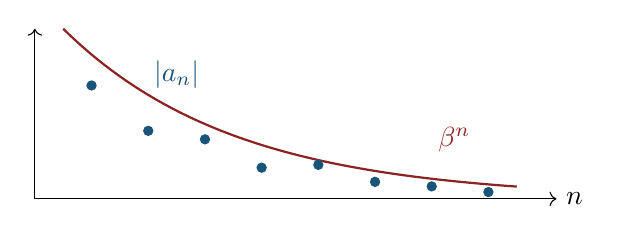
\begin{tikzpicture}[scale=0.72]
    \draw[->] (0,0) -- (9.2,0) node[right]{$n$};
    \draw[->] (0,0) -- (0,3.0);
    \draw[thick,thmcolor,domain=0.5:8.5,samples=60,smooth]
      plot (\x,{3*pow(0.72,\x-0.5)});
    \node[thmcolor] at (7.4,1.05) {$\beta^n$};
    \foreach \x/\y in {1/2.0,2/1.2,3/1.05,4/0.55,5/0.6,6/0.3,7/0.22,8/0.12}
      \fill[defcolor] (\x,\y) circle (2.6pt);
    \node[defcolor] at (2.5,2.2) {$|a_n|$};
  \end{tikzpicture}
  %\end{center}

  \note{
    Before stating the tests, let's recall our benchmark. The geometric
    series, the sum of "x" to the "n", converges exactly when the
    absolute value of "x" is less than one. This single fact is the
    engine behind everything in this section. The key idea is shown in
    the picture. The smooth red curve is the decaying geometric term,
    "beta" to the "n", with "beta" less than one. The blue dots are the
    sizes of our series terms, the absolute values of "a" sub "n". As
    long as the blue dots eventually stay below the red curve, our
    terms are dominated by a convergent geometric series, and the
    comparison test hands us convergence. Both the root test and the
    ratio test work by establishing exactly this domination. Keep this
    picture in mind as we state the root test.
  }
\end{frame}
}

{
\usebackgroundtemplate{%
  
\includegraphics[width=\paperwidth,height=\paperheight,keepaspectratio=false]{chapter_03_bg_02.png}%
}
% =============================================================================
\section{The Root Test}
% =============================================================================

% --- Build 1/2 ---
\begin{frame}{Theorem 3.33: The Root Test}
  \begin{thmblock}{Theorem 3.33 (Root Test)}
    Given $\Sigma a_n$, put
    \[
      \alpha = \limsup_{n \to \infty} \sqrt[n]{|a_n|}.
    \]
  \end{thmblock}

  \note{
    Now the root test. We are given an arbitrary series, the sum of "a"
    sub "n". We form a single number "alpha", defined as the upper
    limit, as "n" goes to infinity, of the "n"th root of the absolute
    value of "a" sub "n". Taking the absolute value first means the
    test applies to series with terms of any sign, even complex terms.
    Taking the upper limit means "alpha" always exists, possibly as
    plus infinity. This one number "alpha" will decide the fate of the
    series. Next, let's see the three cases.
  }
\end{frame}

% --- Build 2/2 ---
\begin{frame}{Theorem 3.33: The Root Test}
  \begin{thmblock}{Theorem 3.33 (Root Test)}
    Given $\Sigma a_n$, put
    $\alpha = \limsup_{n \to \infty} \sqrt[n]{|a_n|}$. Then
    \begin{enumerate}
      \item[(a)] if $\alpha < 1$, $\;\Sigma a_n$ \alert{converges};
      \item[(b)] if $\alpha > 1$, $\;\Sigma a_n$ \alert{diverges};
      \item[(c)] if $\alpha = 1$, the test gives \alert{no information}.
    \end{enumerate}
  \end{thmblock}

  \note{
    Here are the three cases. If "alpha" is less than one, the series
    converges. If "alpha" is greater than one, the series diverges. And
    if "alpha" equals exactly one, the test gives no information at
    all; the series might converge or might diverge, and we must use
    other methods. So the root test is decisive whenever "alpha" avoids
    the single boundary value one. Let's picture these three regions on
    a number line.
  }
\end{frame}

\begin{frame}[c]{Theorem 3.33: Three Regions for $\alpha$}
  \begin{center}
  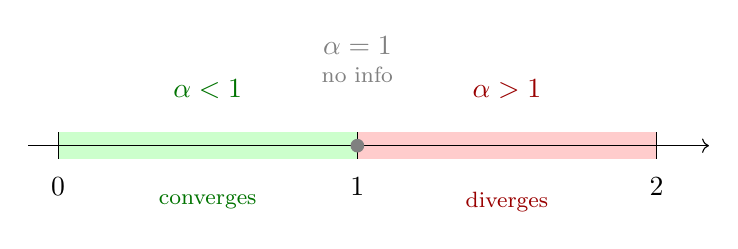
\begin{tikzpicture}[scale=0.95]
    % regions
    \fill[green!20]  (0,-0.18) rectangle (4,0.18);
    \fill[red!20]    (4,-0.18) rectangle (8,0.18);
    \draw[->] (-0.4,0) -- (8.7,0);
    \foreach \x/\l in {0/0,4/1,8/2}
      \draw (\x,0.18)--(\x,-0.18) node[below=3pt]{$\l$};
    \node[green!45!black] at (2,0.75)  {$\alpha < 1$};
    \node[green!45!black] at (2,-0.75) {\footnotesize converges};
    \node[red!60!black]   at (6,0.75)  {$\alpha > 1$};
    \node[red!60!black]   at (6,-0.75) {\footnotesize diverges};
    \fill[gray] (4,0) circle (2.6pt);
    \node[gray,align=center] at (4,1.15) {$\alpha = 1$\\[-2pt]\footnotesize no info};
  \end{tikzpicture}
  \end{center}

  \note{
    This number line summarizes the root test. The value of "alpha"
    sits somewhere on this axis. In the green region to the left of
    one, where "alpha" is less than one, the series converges. In the
    red region to the right of one, where "alpha" is greater than one,
    the series diverges. Exactly at the point one, shown in gray, the
    test is silent. The whole proof comes down to understanding why the
    dividing line falls precisely at one, and the reason is the
    geometric series. Let's prove it.
  }
\end{frame}

\begin{frame}{Proof of Theorem 3.33 --- Strategy}
  \begin{hlbox}
    \textbf{Goal:} Decide convergence of $\Sigma a_n$ from $\alpha$ alone.

    \vspace{0.8em}
    \textbf{Approach --- three cases:}
    \begin{enumerate}
      \item $\alpha < 1$: trap each term below $\beta^n$ for a fixed $\beta < 1$, then compare.
      \item $\alpha > 1$: find infinitely many terms with $|a_n| > 1$, so $a_n \not\to 0$.
      \item $\alpha = 1$: exhibit one convergent and one divergent example.
    \end{enumerate}
  \end{hlbox}

  \note{
    Before the details, here is the plan. There are three cases
    matching the three conclusions. For "alpha" less than one, we trap
    every term, from some point on, below "beta" to the "n" for a fixed
    "beta" between "alpha" and one, then finish with the comparison
    test. For "alpha" greater than one, we produce infinitely many
    terms of absolute value bigger than one, which means the terms
    cannot tend to zero, so the series diverges. For "alpha" equal to
    one, we simply display two example series, one convergent and one
    divergent, both having "alpha" equal to one. Let's carry out the
    first case.
  }
\end{frame}

% --- Build 1/2 ---
\begin{frame}{Proof of Theorem 3.33 --- Case (a): $\alpha < 1$}
  \begin{proofblock}{Case (a): $\alpha < 1$}
    Choose $\beta$ with $\alpha < \beta < 1$. By Theorem 3.17(b),
    there is an integer $N$ such that
    \[
      \sqrt[n]{|a_n|} < \beta \qquad (n \geq N).
    \]
  \end{proofblock}

  \note{
    We begin with "alpha" less than one. Since "alpha" is strictly
    below one, there is room to slip a number "beta" strictly between
    "alpha" and one. Now recall Theorem 3.17, part "b": the upper limit
    "alpha" has the property that only finitely many terms of a
    sequence can exceed any number bigger than "alpha". Since "beta" is
    bigger than "alpha", this means that beyond some index "N", every
    "n"th root of the absolute value of "a" sub "n" is less than
    "beta". Next, we turn this root inequality into a bound on the
    terms themselves.
  }
\end{frame}

% --- Build 2/2 ---
\begin{frame}{Proof of Theorem 3.33 --- Case (a): $\alpha < 1$}
  \begin{proofblock}{Case (a): $\alpha < 1$}
    Choose $\beta$ with $\alpha < \beta < 1$, and $N$ with
    $\sqrt[n]{|a_n|} < \beta$ for $n \geq N$. Raise to the $n$th power:
    \[
      |a_n| < \beta^n \qquad (n \geq N).
    \]
    Since $0 < \beta < 1$, $\;\Sigma \beta^n$ converges. By the
    comparison test, $\;\boxed{\Sigma a_n \text{ converges}.}$
  \end{proofblock}

  \note{
    Raising both sides of that inequality to the "n"th power removes
    the root and gives a clean statement: for every "n" at least "N",
    the absolute value of "a" sub "n" is less than "beta" to the "n".
    But "beta" lies strictly between zero and one, so the geometric
    series of "beta" to the "n" converges. The comparison test now
    finishes the job: our series is dominated, term by term from index
    "N" onward, by a convergent geometric series, so it converges
    absolutely. The first case is complete. Next, the divergent case.
  }
\end{frame}

\begin{frame}{Proof of Theorem 3.33 --- Case (b): $\alpha > 1$}
  \begin{proofblock}{Case (b): $\alpha > 1$}
    By Theorem 3.17, there is a subsequence with
    \[
      \sqrt[n_k]{|a_{n_k}|} \to \alpha > 1.
    \]
    Hence $|a_n| > 1$ for \alert{infinitely many} $n$.\\
    So $a_n \not\to 0$. By Theorem 3.23, $\;\boxed{\Sigma a_n \text{ diverges}.}$
  \end{proofblock}

  \note{
    Now suppose "alpha" is greater than one. By Theorem 3.17, the upper
    limit is actually attained along some subsequence: there is a
    subsequence of indices along which the "n"th root of the absolute
    value of "a" sub "n" converges to "alpha". Since "alpha" exceeds
    one, that root exceeds one for all large members of the
    subsequence, which forces the absolute value of "a" sub "n" itself
    to exceed one for infinitely many "n". But then the terms cannot
    possibly tend to zero. Recall Theorem 3.23: if a series converges,
    its terms must tend to zero. Since that necessary condition fails,
    the series diverges. Next, the borderline case.
  }
\end{frame}

\begin{frame}{Proof of Theorem 3.33 --- Case (c): $\alpha = 1$}
  \begin{proofblock}{Case (c): $\alpha = 1$: no information}
    Consider
    \[
      \sum \frac{1}{n} \quad(\text{diverges}), \qquad
      \sum \frac{1}{n^2} \quad(\text{converges}).
    \]
    For \emph{both}, $\;\alpha = \limsup_{n\to\infty}\sqrt[n]{|a_n|} = 1$
    \quad(since $\sqrt[n]{n} \to 1$).
  \end{proofblock}

  \vspace{0.4em}
  \hl{Same $\alpha$, opposite behavior $\;\Rightarrow\;$ the test cannot decide.}

  \note{
    Finally the borderline. Consider two familiar series: the harmonic
    series, the sum of one over "n", which diverges, and the sum of one
    over "n" squared, which converges. Why is "alpha" equal to one for
    both? Because the "n"th root of "n" tends to one, a standard limit
    we established earlier, and therefore the "n"th root of one over
    "n", and of one over "n" squared, also tend to one. So "alpha"
    equals one in each case. Here we have two series with the very same
    value of "alpha", yet opposite behavior. This proves that when
    "alpha" equals one the root test simply cannot decide the question.
    That completes the proof of the root test. Now let's turn to its
    close relative, the ratio test.
  }
\end{frame}
}

{
\usebackgroundtemplate{%
  
\includegraphics[width=\paperwidth,height=\paperheight,keepaspectratio=false]{chapter_03_bg_03.png}%
}
% =============================================================================
\section{The Ratio Test}
% =============================================================================

% --- Build 1/2 ---
\begin{frame}{Theorem 3.34: The Ratio Test}
  \begin{thmblock}{Theorem 3.34 (Ratio Test)}
    The series $\Sigma a_n$
    \begin{enumerate}
      \item[(a)] \alert{converges} if
        $\displaystyle \limsup_{n \to \infty}
          \left|\frac{a_{n+1}}{a_n}\right| < 1$;
    \end{enumerate}
  \end{thmblock}

  \note{
    The ratio test looks at consecutive terms instead of roots. Here is
    the convergence half. The series converges if the upper limit, as
    "n" goes to infinity, of the absolute value of the ratio of
    consecutive terms is strictly less than one. Intuitively, if each
    term is eventually a definite fraction smaller than the one before
    it, the terms shrink geometrically, just like a geometric series,
    and so the series converges. Notice we use the upper limit here:
    the ratios are allowed to dip and rise, as long as they do not
    creep up to one in the long run. Next, the divergence half.
  }
\end{frame}

% --- Build 2/2 ---
\begin{frame}{Theorem 3.34: The Ratio Test}
  \begin{thmblock}{Theorem 3.34 (Ratio Test)}
    The series $\Sigma a_n$
    \begin{enumerate}
      \item[(a)] \alert{converges} if
        $\displaystyle \limsup_{n \to \infty}
          \left|\frac{a_{n+1}}{a_n}\right| < 1$;
      \item[(b)] \alert{diverges} if
        $\displaystyle \left|\frac{a_{n+1}}{a_n}\right| \geq 1$
        for all $n \geq n_0$, some fixed integer $n_0$.
    \end{enumerate}
  \end{thmblock}

  \note{
    And here is the divergence half. The series diverges if the
    absolute value of the ratio is at least one for every "n" beyond
    some fixed index "n" sub zero. Note the asymmetry with the
    convergence half. For convergence we used the upper limit being
    below one; for divergence we demand that every ratio, from some
    point on, is at least one. This is a stronger requirement than just
    a lower limit being at least one, and the proof will show why we
    phrase it this way. Next, an important warning.
  }
\end{frame}

\begin{frame}{Theorem 3.34: A Warning}
  \begin{remblock}{Note}
    Knowing $\;\lim\limits_{n\to\infty} \left|\dfrac{a_{n+1}}{a_n}\right| = 1\;$
    implies \alert{nothing} about convergence.
  \end{remblock}

  \vspace{0.5em}
  \begin{hlbox}
    Once again $\;\sum \dfrac{1}{n}\;$ and $\;\sum \dfrac{1}{n^2}\;$ both have ratio limit $1$,
    yet one diverges and the other converges.
  \end{hlbox}

  \note{
    A warning, exactly parallel to the root test. If the limit of the
    ratio equals one, the ratio test tells us nothing. The same two
    series make the point: for both the harmonic series and the sum of
    one over "n" squared, the ratio of consecutive terms tends to one,
    yet one diverges and the other converges. So a ratio limit of one
    is genuinely inconclusive. Next, let's prove the ratio test.
  }
\end{frame}

% --- Build 1/2 ---
\begin{frame}{Proof of Theorem 3.34 --- Case (a): convergence}
  \begin{proofblock}{Case (a): $\limsup |a_{n+1}/a_n| < 1$}
    Pick $\beta < 1$ and $N$ with
    $\left|\frac{a_{n+1}}{a_n}\right| < \beta$ for $n \geq N$. Cascading:
    \[
      |a_{N+1}| < \beta|a_N|,\quad
      |a_{N+2}| < \beta^2|a_N|,\quad
      \dots,\quad
      |a_{N+p}| < \beta^p|a_N|.
    \]
  \end{proofblock}

  \note{
    Suppose the upper limit of the ratio is below one. Then we can
    choose a number "beta" still below one but above that upper limit,
    and an index "N" so that every ratio past "N" is less than "beta".
    Now we cascade. The term at "N" plus one is less than "beta" times
    the term at "N". The term at "N" plus two is less than "beta" times
    that, hence less than "beta" squared times the term at "N".
    Continuing this telescoping pattern, the term at "N" plus "p" is
    less than "beta" to the "p" times the absolute value of the term at
    "N". Next, we rewrite this as a single clean bound.
  }
\end{frame}

% --- Build 2/2 ---
\begin{frame}{Proof of Theorem 3.34 --- Case (a): convergence}
  \begin{proofblock}{Case (a): $\limsup |a_{n+1}/a_n| < 1$}
    With $n > N$, the cascade becomes
    \[
      |a_n| < |a_N|\,\beta^{-N} \cdot \beta^n \qquad (n > N).
    \]
    The factor $|a_N|\beta^{-N}$ is a \alert{constant}. Since
    $\Sigma \beta^n$ converges,
    $\;\boxed{\Sigma a_n \text{ converges}}$ by comparison.
  \end{proofblock}

  \note{
    Setting "n" equal to "N" plus "p", the cascade collapses into a
    single inequality: for every "n" greater than "N", the absolute
    value of "a" sub "n" is less than a fixed constant, namely the
    absolute value of "a" sub "N" times "beta" to the minus "N",
    multiplied by "beta" to the "n". The crucial point is that the
    constant does not depend on "n"; only the "beta" to the "n" factor
    changes. So the terms are dominated by a constant multiple of the
    geometric series of "beta" to the "n", which converges because
    "beta" is below one. The comparison test gives convergence. The
    first case is done. Next, divergence.
  }
\end{frame}

\begin{frame}{Proof of Theorem 3.34 --- Case (b): divergence}
  \begin{proofblock}{Case (b): $|a_{n+1}| \geq |a_n|$ for $n \geq n_0$}
    The sizes of the terms never decrease past $n_0$:
    \[
      |a_{n_0}| \leq |a_{n_0+1}| \leq |a_{n_0+2}| \leq \cdots
    \]
    Hence $a_n \not\to 0$, so $\;\boxed{\Sigma a_n \text{ diverges}.}$
  \end{proofblock}

  \note{
    For divergence, suppose that, from some index "n" sub zero on, each
    term is at least as large in absolute value as the one before it.
    Then the sizes of the terms never decrease from that point on. A
    sequence whose terms never shrink in size cannot tend to zero,
    unless they were already zero, which would make the ratio
    undefined. But recall the necessary condition for convergence from
    Theorem 3.23: the terms of any convergent series must tend to zero.
    That condition fails here, so the series diverges. Notice how crude
    this is: we never even looked at how big the ratio is, only that it
    stays at least one. That completes the proof of the ratio test.
    Next, some examples that reveal a real difference between the two
    tests.
  }
\end{frame}
}

{
\usebackgroundtemplate{%
  
\includegraphics[width=\paperwidth,height=\paperheight,keepaspectratio=false]{chapter_03_bg_04.png}%
}
% =============================================================================
\section{Examples and Remarks}
% =============================================================================

% --- Build 1/2 ---
\begin{frame}{Example 3.35(a): Root Wins, Ratio Fails}
  \begin{exblock}{Example 3.35(a)}
    \[
      \tfrac{1}{2} + \tfrac{1}{3}
      + \tfrac{1}{2^2} + \tfrac{1}{3^2}
      + \tfrac{1}{2^3} + \tfrac{1}{3^3}
      + \tfrac{1}{2^4} + \tfrac{1}{3^4} + \cdots
    \]
    Two geometric series --- powers of $\tfrac12$ and powers of $\tfrac13$ ---
    \alert{interleaved}.
  \end{exblock}

  \note{
    Here is a revealing example. The series interleaves two geometric
    series: the powers of one half and the powers of one third, taken
    in the order one half, one third, one half squared, one third
    squared, and so on. Each individual piece is a perfectly nice
    convergent geometric series, but by shuffling them together we
    create a series whose consecutive ratios behave wildly. Let's
    compute the relevant quantities and see what each test says.
  }
\end{frame}

% --- Build 2/2 ---
\begin{frame}{Example 3.35(a): Root Wins, Ratio Fails}
  \begin{exblock}{Example 3.35(a)}
    \[
      \liminf \tfrac{a_{n+1}}{a_n} = 0, \qquad
      \limsup \tfrac{a_{n+1}}{a_n} = +\infty,
    \]
    \[
      \liminf \sqrt[n]{a_n} = \tfrac{1}{\sqrt{3}}, \qquad
      \limsup \sqrt[n]{a_n} = \tfrac{1}{\sqrt{2}}.
    \]
  \end{exblock}

  \vspace{0.3em}
  \begin{hlbox}
    \textbf{Root test:} $\alpha = 1/\sqrt{2} < 1 \;\Rightarrow\;$ \alert{converges}.\\
    \textbf{Ratio test:} $\limsup = +\infty \;\Rightarrow\;$ no conclusion.
  \end{hlbox}

  \note{
    Look at the four numbers. The ratios swing all the way from a lower
    limit of zero up to an upper limit of plus infinity, because going
    from a one third term to the next one half term the ratio blows up.
    So the ratio test is helpless here; its upper limit is infinite,
    well above one. The roots, however, are tame: the "n"th roots stay
    between one over root three and one over root two. The root test
    uses the upper limit, one over root two, which is less than one, so
    the root test cleanly concludes convergence. The root test
    succeeds exactly where the ratio test fails. Next, a second example
    with the same lesson.
  }
\end{frame}

\begin{frame}{Example 3.35(b): Same Lesson}
  \begin{exblock}{Example 3.35(b)}
    \[
      \tfrac{1}{2} + 1 + \tfrac{1}{8} + \tfrac{1}{4}
      + \tfrac{1}{32} + \tfrac{1}{16}
      + \tfrac{1}{128} + \tfrac{1}{64} + \cdots
    \]
    \[
      \liminf \tfrac{a_{n+1}}{a_n} = \tfrac{1}{8}, \qquad
      \limsup \tfrac{a_{n+1}}{a_n} = 2, \qquad
      \lim \sqrt[n]{a_n} = \tfrac{1}{2}.
    \]
  \end{exblock}

  \vspace{0.3em}
  \begin{hlbox}
    \textbf{Root test:} $\tfrac12 < 1 \;\Rightarrow\;$ \alert{converges}.\\
    \textbf{Ratio test:} $\limsup = 2 > 1 \;\Rightarrow\;$ no conclusion.
  \end{hlbox}

  \note{
    The second example tells the same story in a slightly different
    way. Here the powers of one half are listed two at a time, with
    each pair in swapped order, so a smaller term is always followed by
    a larger one. The lower limit of the ratios is one eighth and the
    upper limit is two. Since
    the upper limit, two, is bigger than one, the ratio test once again
    gives no conclusion. But the "n"th roots actually converge, to one
    half. Since one half is below one, the root test again concludes
    convergence. Two examples, one moral: the root test can decide
    cases the ratio test cannot. Let's make that observation precise.
  }
\end{frame}

% --- Build 1/2 ---
\begin{frame}{Remark 3.36: Comparing the Two Tests}
  \begin{remblock}{Remark 3.36}
    The \alert{ratio test} is frequently \emph{easier to apply} ---
    computing ratios is usually simpler than computing $n$th roots.
  \end{remblock}

  \note{
    Remark 3.36 weighs the two tests against each other. In day to day
    practice, the ratio test is frequently easier to apply, simply
    because computing a ratio of consecutive terms is usually less work
    than computing an "n"th root and then its limit. So for many
    standard series the ratio test is the convenient first choice. But
    ease of use is not the whole story. Next, the deeper comparison.
  }
\end{frame}

% --- Build 2/2 ---
\begin{frame}{Remark 3.36: Comparing the Two Tests}
  \begin{remblock}{Remark 3.36}
    The \alert{ratio test} is frequently \emph{easier to apply} ---
    computing ratios is usually simpler than computing $n$th roots.

    \medskip
    The \alert{root test} has \emph{wider scope}:
    \begin{itemize}
      \item whenever the ratio test shows convergence, so does the root test;
      \item whenever the root test is inconclusive, so is the ratio test.
    \end{itemize}
    Neither test is subtle about \emph{divergence}: both rely on $a_n \not\to 0$.
  \end{remblock}

  \note{
    The root test, on the other hand, has wider scope. Whenever the
    ratio test proves convergence, the root test proves it too; and
    whenever the root test fails to decide, the ratio test also fails.
    So the root test is strictly more powerful, never weaker. Our two
    examples illustrated exactly this. We will prove this relationship
    in a moment. One more remark: neither test is subtle when it comes
    to divergence. Both detect divergence only in the crude way, by
    noticing that the terms fail to tend to zero. Next, the theorem
    that justifies the comparison.
  }
\end{frame}
}

{
\usebackgroundtemplate{%
  
\includegraphics[width=\paperwidth,height=\paperheight,keepaspectratio=false]{chapter_03_bg_05.png}%
}
% =============================================================================
\section{Root vs.\ Ratio}
% =============================================================================

\begin{frame}{Theorem 3.37: Roots Squeezed Between Ratios}
  \begin{thmblock}{Theorem 3.37}
    For any sequence $\{c_n\}$ of \emph{positive} numbers,
    \[
      \liminf_{n \to \infty} \frac{c_{n+1}}{c_n}
        \;\leq\; \liminf_{n \to \infty} \sqrt[n]{c_n},
    \]
    \[
      \limsup_{n \to \infty} \sqrt[n]{c_n}
        \;\leq\; \limsup_{n \to \infty} \frac{c_{n+1}}{c_n}.
    \]
  \end{thmblock}

  \note{
    Here is the theorem behind the remark. For any sequence of positive
    numbers "c" sub "n", two inequalities hold. The lower limit of the
    ratios is at most the lower limit of the "n"th roots, and the upper
    limit of the "n"th roots is at most the upper limit of the ratios.
    In words, the root quantities are always squeezed between the ratio
    quantities. Let's see this as a picture before proving it.
  }
\end{frame}

\begin{frame}{Theorem 3.37: The Squeeze, Pictured}
  \begin{center}
  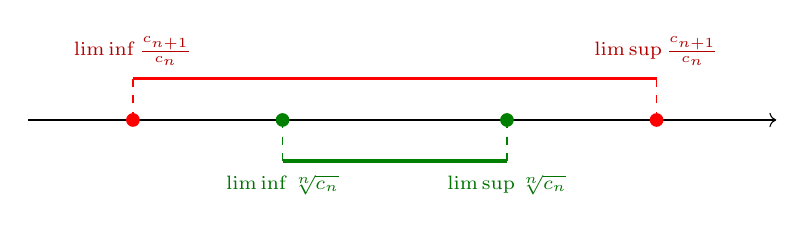
\begin{tikzpicture}[scale=0.95]
    \draw[->] (-0.4,0) -- (9.6,0);
    % ratio interval (outer, red)
    \draw[red,very thick] (1,0.55)--(8,0.55);
    \fill[red] (1,0) circle (2.6pt);
    \fill[red] (8,0) circle (2.6pt);
    \draw[red,dashed] (1,0)--(1,0.55);
    \draw[red,dashed] (8,0)--(8,0.55);
    \node[red!70!black,above,font=\scriptsize] at (1,0.6)
      {$\liminf \frac{c_{n+1}}{c_n}$};
    \node[red!70!black,above,font=\scriptsize] at (8,0.6)
      {$\limsup \frac{c_{n+1}}{c_n}$};
    % root interval (inner, green)
    \draw[green!50!black,very thick] (3,-0.55)--(6,-0.55);
    \fill[green!50!black] (3,0) circle (2.6pt);
    \fill[green!50!black] (6,0) circle (2.6pt);
    \draw[green!50!black,dashed] (3,0)--(3,-0.55);
    \draw[green!50!black,dashed] (6,0)--(6,-0.55);
    \node[green!45!black,below,font=\scriptsize] at (3,-0.6)
      {$\liminf \sqrt[n]{c_n}$};
    \node[green!45!black,below,font=\scriptsize] at (6,-0.6)
      {$\limsup \sqrt[n]{c_n}$};
  \end{tikzpicture}
  \end{center}

  \vspace{0.3em}
  \hl{The \alert{root} interval (green) sits \emph{inside} the \alert{ratio} interval (red).}

  \note{
    This picture shows the squeeze. On the number line, the two ratio
    quantities, the lower limit and the upper limit of the ratios, sit
    on the outside, drawn in red. The two root quantities, the lower
    and upper limits of the "n"th roots, sit on the inside, drawn in
    green. The interval determined by the root test is always
    contained inside the interval determined by the ratio test. This is
    exactly why the root test has wider scope: its decisive interval is
    narrower and better placed. Now let's prove the second inequality.
  }
\end{frame}

\begin{frame}{Proof of Theorem 3.37 --- Setup}
  \begin{proofblock}{Setup}
    Prove the \emph{second} inequality (the first is similar). Put
    $\alpha = \limsup_{n\to\infty} \frac{c_{n+1}}{c_n}$.
    \begin{itemize}
      \item If $\alpha = +\infty$: Nothing to prove.
      \item If $\alpha < +\infty$: Choose any $\beta > \alpha$.\\
        Then there is $N$ with $\dfrac{c_{n+1}}{c_n} \leq \beta$ for $n \geq N$.
    \end{itemize}
  \end{proofblock}

  \note{
    We prove the second inequality; the first is entirely similar. Let
    "alpha" denote the upper limit of the ratios. If "alpha" is plus
    infinity, the inequality holds automatically, since nothing can
    exceed infinity, and there is nothing to prove. So assume "alpha"
    is finite, and choose any number "beta" larger than "alpha". By the
    meaning of the upper limit, only finitely many ratios can exceed
    "beta", so there is an index "N" beyond which every ratio is at
    most "beta". Next, we cascade these inequalities, just as in the
    ratio test proof.
  }
\end{frame}

\begin{frame}{Proof of Theorem 3.37 --- The Cascade}
  \begin{proofblock}{Cascade}
    For $k = 0, 1, \dots, p-1$: $\;\;c_{N+k+1} \leq \beta\, c_{N+k}$.
    Multiplying all of these:
    \[
      c_{N+p} \leq \beta^p c_N,
      \qquad\text{i.e.}\qquad
      c_n \leq c_N \beta^{-N} \cdot \beta^n \quad (n \geq N).
    \]
  \end{proofblock}

  \note{
    Past the index "N", each term is at most "beta" times the previous
    term. Writing this out for "k" running from zero up to "p" minus
    one, we get a chain of inequalities. Multiplying all of them
    together, the intermediate terms cancel in pairs, and we are left
    with: the term at "N" plus "p" is at most "beta" to the "p" times
    the term at "N". Setting "n" equal to "N" plus "p", this says "c"
    sub "n" is at most the constant "c" sub "N" times "beta" to the
    minus "N", multiplied by "beta" to the "n", valid for every "n" at
    least "N". Next, we extract the "n"th root.
  }
\end{frame}

\begin{frame}{Proof of Theorem 3.37 --- Conclusion}
  \begin{proofblock}{Conclusion}
    Take $n$th roots: $\;\sqrt[n]{c_n} \leq \sqrt[n]{c_N \beta^{-N}} \cdot \beta$.\\
    Since $\sqrt[n]{c_N\beta^{-N}} \to 1$, by Theorem 3.20(b)
    \begin{equation}
      \limsup_{n\to\infty} \sqrt[n]{c_n} \leq \beta. \tag{18}
    \end{equation}
    True for \emph{every} $\beta > \alpha$, hence
    $\;\boxed{\limsup_{n\to\infty}\sqrt[n]{c_n} \leq \alpha.}$
  \end{proofblock}

  \note{
    Now take the "n"th root of both sides. The right side becomes the
    "n"th root of the constant, times "beta". As "n" grows, the "n"th
    root of any fixed positive constant tends to one. Therefore,
    passing to the upper limit and using Theorem 3.20, part "b", we
    obtain inequality eighteen: the upper limit of the "n"th roots is
    at most "beta". But "beta" was an arbitrary number greater than
    "alpha". Since the inequality holds for every such "beta", it must
    also hold for "alpha" itself, giving the upper limit of the "n"th
    roots is at most "alpha". That is exactly the second inequality,
    and the proof is complete. Let's summarize.
  }
\end{frame}
}

{
\usebackgroundtemplate{%
  
\includegraphics[width=\paperwidth,height=\paperheight,keepaspectratio=false]{chapter_03_bg_06.png}%
}
% =============================================================================
\section{Summary}
% =============================================================================

% --- Build 1/3 ---
\begin{frame}{Summary}
  \begin{hlbox}
    \textbf{Key takeaways:}
    \begin{itemize}
      \item \alert{Root test (3.33):} with $\alpha = \limsup\sqrt[n]{|a_n|}$:
        converges if $\alpha < 1$, diverges if $\alpha > 1$,
        inconclusive if $\alpha = 1$.
    \end{itemize}
  \end{hlbox}

  \note{
    Let's gather the key points. First, the root test. Form the upper
    limit of the "n"th root of the absolute value of "a" sub "n", and
    call it "alpha". If "alpha" is below one the series converges, if
    above one it diverges, and if exactly one the test is
    inconclusive. Next, the ratio test.
  }
\end{frame}

% --- Build 2/3 ---
\begin{frame}{Summary}
  \begin{hlbox}
    \textbf{Key takeaways:}
    \begin{itemize}
      \item \alert{Root test (3.33):} with $\alpha = \limsup\sqrt[n]{|a_n|}$:
        converges if $\alpha < 1$, diverges if $\alpha > 1$,
        inconclusive if $\alpha = 1$.
      \item \alert{Ratio test (3.34):} converges if $\limsup|a_{n+1}/a_n| < 1$,
        diverges if $|a_{n+1}/a_n| \geq 1$ eventually.
    \end{itemize}
  \end{hlbox}

  \note{
    Second, the ratio test. The series converges if the upper limit of
    the absolute ratio of consecutive terms is below one, and diverges
    if that ratio stays at least one from some point on. The ratio test
    is usually easier to compute. Both tests work by secretly comparing
    the series to a geometric series. Next, the relationship between
    them.
  }
\end{frame}

% --- Build 3/3 ---
\begin{frame}{Summary}
  \begin{hlbox}
    \textbf{Key takeaways:}
    \begin{itemize}
      \item \alert{Root test (3.33):} with $\alpha = \limsup\sqrt[n]{|a_n|}$:
        converges if $\alpha < 1$, diverges if $\alpha > 1$,
        inconclusive if $\alpha = 1$.
      \item \alert{Ratio test (3.34):} converges if $\limsup|a_{n+1}/a_n| < 1$,
        diverges if $|a_{n+1}/a_n| \geq 1$ eventually.
      \item \alert{Theorem 3.37:} roots are squeezed between ratios ---
        the root test has \emph{wider scope}.
    \end{itemize}

    \vspace{0.8em}
    \textbf{Coming up next:} Power Series.
  \end{hlbox}

  \note{
    Third, Theorem 3.37 tells us the root quantities are always
    squeezed between the ratio quantities. The practical consequence is
    that the root test has wider scope: anything the ratio test
    settles, the root test settles too, but not the other way around.
    Coming up next, we apply these ideas to power series, where the
    root test will pin down the radius of convergence, the interval on
    which a power series defines a function. See you in the next
    section.
  }
\end{frame}
}

\end{document}
